\chapter{Podstawy teoretyczne}

\section{Rozpoznawanie emocji}

Rozpoznawanie emocji w dialogach koncentruje się na wydobyciu emocji przekazanej w rozmowie pomiędzy co najmniej dwoma rozmówcami. Problem ten stawia bardzo dużo wyzwań, takich jak obecność sarkazmu w rozmowie, przesunięcie emocji do kolejnych wypowiedzi tego samego rozmówcy oraz uchwycenie szerszego kontekstu pomiędzy wypowiedziami różnych rozmówców. Dużym plusem w tej dziedzinie jest bardzo dobra dostępność do danych, które pochodzą z platform społecznościowych takich jak Facebook, Youtube, Reddit, Twitter \cite{poria2019emotion}. Poprzez łatwą dostępność do danych rozpoznawanie emocji w rozmowie staje się coraz bardziej popularne, a trudność tego problemu stwarza coraz to bardziej odległe granice co sprowadza się do wysokiego zainteresowania tą dziedziną przetwarzania języka naturalnego (ang. \textit{natural language processing}).

Bardzo ważnym elementem w rozpoznawaniu emocji jest możliwość zrozumienia danego przekazu w kontekście, od którego może zależeć rodzaj emocji. Szczególnie trudnym przypadkiem jest zrozumienie i zapamiętanie kontekstu w konwersacji, co jak pokazuje \cite{zhong2019knowledgeenriched}, może okazać się kluczowym czynnikiem skuteczności rozpoznawania emocji. Do uzyskania satysfakcjonujących wyników nie wystarczają tradycyjne metody uczenia maszynowego lub najbardziej podstawowe architektury sieci neuronowych. Modele te wykorzystują zaawansowane techniki architektury transformera (ang. \textit{the Transformer}) \cite{vaswani2017attention} które korzystają z podejścia mającego na celu poprawę modelowania sekwencja do sekwencji (ang. \textit{Seq2Seq}) poprzez samoobserwację (ang. \textit{self-attention}) i kodowanie pozycji (ang. \textit{positional encoding}).

\section{Modele emocji}

Aby dobrze zrozumieć postawiony problem niezbędne będzie określenie czym są emocje. Wszyscy ludzie posiadają wrodzony zestaw podstawowych emocji, które można rozpoznać za pomocą gestów, czynów lub wypowiadanych słów. Możemy wyróżnić dyskretne emocje aby móc odróżnić je od siebie. Istnieje kilka definicji różnych modeli emocji, jednym z nich jest model zaproponowany przez Paula Ekmana \cite{ekman1993facial}.  Paul wraz ze współpracownikami stwierdzili, że istnieje sześć podstawowych emocji: gniew, obrzydzenie, strach, szczęście, smutek i zaskoczenie, a z każdą z tych emocji związane są jakieś cechy. Dzięki temu można wyrazić emocje w różnym stopniu a każda z nich jest zdefiniowana jako dyskretna kategoria co pozwala na dość łatwą klasyfikację konkretnej emocji.

Kolejną definicję modelu emocji przedstawił Robert Plutchik, który podzielił emocje na osiem podstawowych typów, z których każdy ma drobniejsze podtypy pokrewne \cite{plutchik1982psychoevolutionary}, zaprezentowane na rysunku \ref{rys:plutchik_wheel} za pomocą koła emocji. Reprezentuje on emocje jako koncentryczne kręgi, wewnętrzne części odpowiadają za podstawowe emocje a te zewnętrzna za bardziej złożone. Model ten jest dyskretny, lecz widać w nim pewne zależności i podobieństwa pomiędzy sąsiadującymi częściami koła emocji. Budowa ta wynika ze złożoności emocji i możliwości wyrażania ich intensywności.   

\begin{figure}[t]
\centering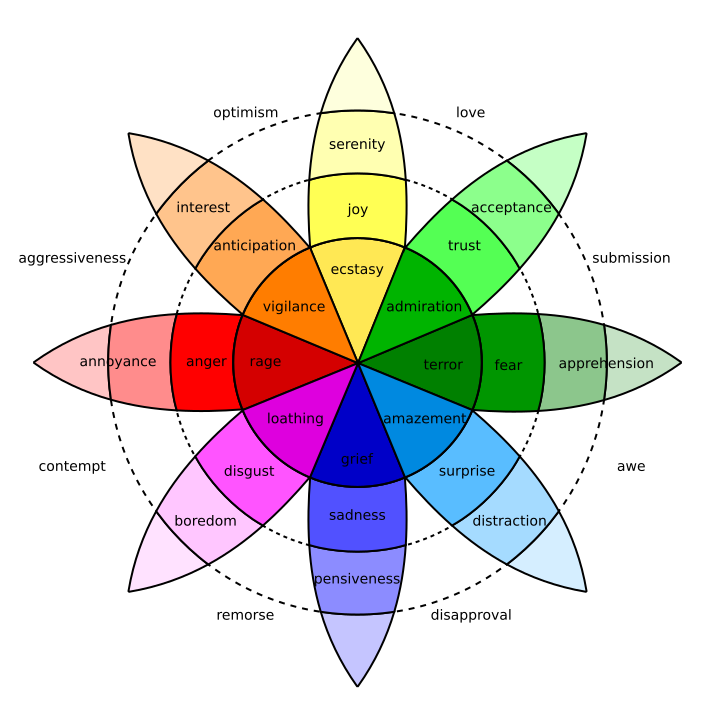
\includegraphics[width=10cm]{figures/plutchik-wheel.png}
\fcmfcaption{Koło emocji Plutchika \cite{plutchik1982psychoevolutionary}.}\label{rys:plutchik_wheel}
\end{figure}

Podsumowując wymienione modele emocji możemy wydzielić dwa główne typy: kategoryczne oraz wymiarowe. Modele wymiarowe mapują emocję w sposób ciągły na wektory. Modele kategoryczne klasyfikują emocję do konkretnej emocji dyskretnej, np. jednej z wybranego modelu emocji Ekmana lub Plutchika. Modele kategoryczne mają pewne wady, jedną z nich jest brak możliwości opisania innych emocji oraz utrudnione opisywanie emocji złożonej z kilku różnych podtypów zdefiniowanych w dyskretnym modelu. Drugą wadą jest brak możliwości porównywania emocji co umożliwiłby model wymiarowy, za pomocą porównywania dwóch wektorów. Wybór odpowiedniego modelu emocji nie jest łatwy i jednocześnie jest bardzo ważnym elementem do późniejszej klasyfikacji emocji. Decydując się na kategoryczny typ emocji z jednej strony mamy prosty model Ekmana który nie jest w stanie zamodelować złożonych emocji. Z drugiej strony w modelu Plutchika może być bardzo trudno rozróżnić drobnoziarniste emocje od siebie. Wybór ten należy zatem dokonać mając na uwadze wielkość oraz jakość zbioru danych.